% TeX encoding = utf8
% TeX spellcheck = pl_PL 
\documentclass[a4paper, 11pt]{article}
\usepackage[utf8]{inputenc}
\usepackage[polish]{babel}
\usepackage{polski}
\usepackage{float}
\usepackage{graphicx}
\usepackage{listings}
\usepackage{amsfonts}
\usepackage{geometry}
\usepackage{multicol}
\usepackage{latexsym}
\usepackage{enumerate}
\usepackage{hyperref}
\usepackage{wrapfig}
\usepackage{color} %red, green, blue, yellow, cyan, magenta, black, white
\definecolor{mygreen}{RGB}{28,172,0} % color values Red, Green, Blue
\definecolor{mylilas}{RGB}{170,55,241}

\author{Kamil Foryszewski}
\title{Dokumentacja projektu laboratoryjnego numer 3 przedmiot MNUM}
\frenchspacing

\newgeometry{tmargin=2cm, bmargin=2cm, lmargin=2cm, rmargin=2cm}
\pagestyle{empty}


\begin{document}

\lstset{language=Matlab,%
    basicstyle=\color{red},
    breaklines=true,%
    morekeywords={matlab2tikz},
    keywordstyle=\color{blue},%
    morekeywords=[2]{1}, keywordstyle=[2]{\color{black}},
    identifierstyle=\color{black},%
    stringstyle=\color{mylilas},%
    commentstyle=\color{mygreen},%
    showstringspaces=false,
    numbers=right,%
    numberstyle={ \color{black}},% size of the numbers
    numbersep=5pt, % this defines how far the numbers are from the text
    emph=[1]{for,endfor,endwhile,endfunction,endif,break},emphstyle=[1]\color{blue}, %some words to emphasise
    emph=[2]{,.}, emphstyle=[2]\color{yellow},%
}

\maketitle
\tableofcontents

\section{Zadanie 1}

\subsection{Polecenie}
Proszę znaleźć wszystkie zera funkcji
\begin{center}
$f(x) = 1.4*sin(x)-e^{x}=6*x-0.5$
\end{center}
w przedziale $[-5,5]$, używając dla każdego zera programu z implementacją \\
a) metody bisekcji\\
b) metody siecznych\\
c) metody Newtona\\
 

\subsection{Metoda bisekcji}
\subsubsection{Opis teoretyczny}
Teoretyczny zarys metody bisekcji możemy przybliżyć poniższym algorytmem:
\begin{enumerate}
  \item Począwszy od przedziału startowego $[a,b]$ = $[a_{0},b_{0}]$ obliczamy środek przedziału $c_{n}$\\
  	\begin{center}
  	$c_{n} = \frac{a_{n}+b_{n}}{2}$\\
	\end{center}
  i obliczamy wartość $f(x)$ w tym punkcie. 
  \item Obliczamy iloczyny $f(a_{n})*f(c_{n})$ oraz $f(b_{n})*f(c_{n})$ i jako nowy przedział $[a_{n=1},b_{n+1}]$
  wybieramy argumenty tego iliczynu którego wartość jest ujemna. 
\end{enumerate} 
Kroki te powtarzamy aż do mementu uzyskania $f(c_{n})<\delta$ gdzie $\delta$ to oczekiwana dokładność rozwiązania. W przypadku "płaskich"  funkcji warto też konrtolować długość rozpatrywanego przedziału. 
Dokładność wyniku zalezy jedynie od ilości iteracji dlatego metoda jest zbierzna liniowo z ilorazem zbierzności 0.5, co czyni ją stosunkowo wolno zbierzną w przypadku wyboru szerokiego przedziału początkowego. 



\subsubsection{Realizacja w programie Matlab}
\begin{lstlisting}
%funkcja wyznaczajaca zera funkcji metoda bisekcji
function bzeropoint = bisection(fun,l,r,iter)
%Dane wejsciowe:	l,r - lewa i prawa sterona przedzialu poszukiwan
%			fun - funkcja 
%			iter - maksymalna liczba uteracji
%Dane wyjsciowe: zerospoint - wyznaczone miejsce zerowe
  a = l; 
  b = r;
  fa =feval(fun,a);     %  Wartosci poczatkowe f(a) i f(b)
  fb =feval(fun,b);
  for k=1:iter
    xm = a + 0.5*(b-a);    %  Poprawne obliczenie srodka przedzialu
    fm = feval(fun,xm);      %  f(x) w srodku przedzialu
    fprintf('%3d %12.16f %12.16f %12.16f %12.3e\n',k,a,xm,b,fm);
    if(fm == 0)
        return
    end
    if sign(fm)==sign(fa)    %  Zero lezy w przedziale [xm,b], zamiana a
        a = xm;
        fa = fm;
    else                     %  Zero lezy w przedziale [a,xm], zamiana b
        b = xm;
        fb = fm;
    end
  end
  bzeropoint = xm; 
  return
end
\end{lstlisting}

\subsection{Metoda siecznych}
\subsubsection{Opis teoretyczny}
Teoretyczny zarys metody siecznych możemy przybliżyć poniższym algorytmem:
\begin{enumerate}
  \item Począwszy od przedziału startowego $[a,b]$ = $[a_{0},b_{0}]$ obliczamy punkt $\delta x_{n}$ jako miejcse przecięcia siecznej funkcji przechodzącej prze punkty $[a_{n},b_{n}]$ gdzie $\delta x_{n}=\frac{f(x_{n})(x_{n}-x_{n-1})}{f(x_{n})-f(x_{n-1})}$
  \item Nastpepnie nowy przedział oznaczamy $x_{n+1}=x_{n}-\delta x_{n}$ 
\end{enumerate} 
Kroki te powtarzamy aż do mementu uzyskania $f(c_{n})<\delta$ gdzie $\delta$ to oczekiwana dokładność rozwiązania. Rząd zbierzności metody siecznych wynosi $(1+sqrt(5))/2$ co jest w przybliżeniu równe $1.618$. 
Jest więc ona dużo szybsza od metody bisekcji, jednak jest zbierzna jedynie lokalnie. Jeżeli ine zadbamy o wybór odpowiedniego przedziału początkowego może okazać się w ogóle nie zbieżna.


\subsubsection{Realizacja w programie Matlab}
\begin{lstlisting}
%funkcja obliczajaca zera funkcji metoda siecznych
function szeropoint = secant(fun,l,r,iter)
%Dane wejsciowe:	l.r - lewa i prawa sterona przedzialu poszukiwan
%			fun - funkcja 
%			iter - maksymalna liczba uteracji
%Dane wyjsciowe: zerospoint - wwyznaczone miejsce zerowe
  a = l;
  b = r;
  fa = feval(fun,a); %wartosc funkcji w punkcie start.
  for k = 1:iter
    fb = feval(fun,b);
    dx = fb * (b-a) / (fb-fa); %wyznaczenie przeciecia sieczna
    xm = b-dx; %zawezenie przedzialu
    if(isnan(xm))
        return
    end
    a = b;
    b = xm;
    fa = fb;
    szeropoint = b;
    fprintf('%3d %12.16f %12.16f %12.16f %12.3e\n',k,a,xm,b,dx);
    if(fb == 0) %dodatkowy warunek zakonczenia wykonywania
        return
    end
  end
end
\end{lstlisting}

\subsection{Metoda Newtona}
\subsubsection{Opis teoretyczny}
Metoda Newtona polega na wyznaczeniu częściowego (uciętego) rozwinięcia w szereg Taylora danej funkcji, które możemy trakować jak liniowe przybliżenie funkcji według wzoru:\
  	\begin{center}
  	$f(x) \approx f(x_{n})+f'(x_{n})(x-x_{n})$
	\end{center}
Nastepnie wyznaczamy kolejne punkty iteracji poprzez przywórnanie do zera otrzymanej aproksymacji:\\
\begin{center}
$f(x_{n})+f'(x_{n})(x_{n+1}-x_{n}) = 0$
\end{center}
Prowadzi to do zależności iteracyjnej danej następującym wzorem:\\
\begin{center}
$x_{n+1} = x_{n}-\frac{f(x_{n})}{f'(x_{n})}$
\end{center}
Metoda Newtona jest zbierzna jedynie lokalnie, ponieważ wyznaczjąc styczną do wykresu w danym punkcie możemy w przypadku ujemnego znaku pochodnej dojsć do rozbierzności. Dla przypadków pochodnej większej od zera metoda jest zbierzna kwadratowo. Rząd zbierzności wynosi 2.

\subsubsection{Realizacja w programie Matlab}
\begin{lstlisting}
%funkcja obliczajaca zera funkcji metoda Newtona
function nzeropoint = newton(fun,l,iter)
%Dane wejsciowe:	l prawa sterona przedzialu poszukiwan
%			fun - funkcja 
%			iter - maksymalna liczba uteracji
%Dane wyjsciowe: zerospoint - wyznaczone miejsce zerowe
    
  x0 = l; 
  for k = 1:iter
    [fold, fpold] = feval(fun,x0); 
    dx = fold / fpold; %wyznaczenie przyrostu funkcji
    x0 = x0 - dx;
    fprintf('%3d %12.16f %12.16f %12.3e\n',k,x0,dx,fold);
    if(fold == 0)
        return
    end
	if fold==0 %dodatkowy warunek zatrzumania
        nzeropoint = x0;
        break; 
     end
  end
end
\end{lstlisting}

\subsection{Analiza danych wejściowych}
W celu wyznaczenia przedziałów izolacji miejsc zerowych został wykorsyztany algorytm opisany w skrypcie prof. Tatjewskiego. Wstępna analiza danych rozpoczyna się od wygenerowania wykresu funkcji w danym przedziale i na tej podstawie wyboru przedziału startowego dla algorytmu. Nastepnie w podanycm przedziale w pętli badany jest znak iloczynu funkcji w punktach graniczynych. Jezeli jest on ujemny, oznacza to występowanie miejsca zerowego w danycm przedziale. Jeżeli nie, to przedział jest rozszerzany do momentu przekroczenia przedziału danego w zadaniu. 
Poniżej wykres funkcji z zaznaczonymi przedziałami izolacji wyznaczonymi przez algorytm. 

\begin{figure}[H]
\caption{Wykres z zaznaczonymi przedziałami startowymi}
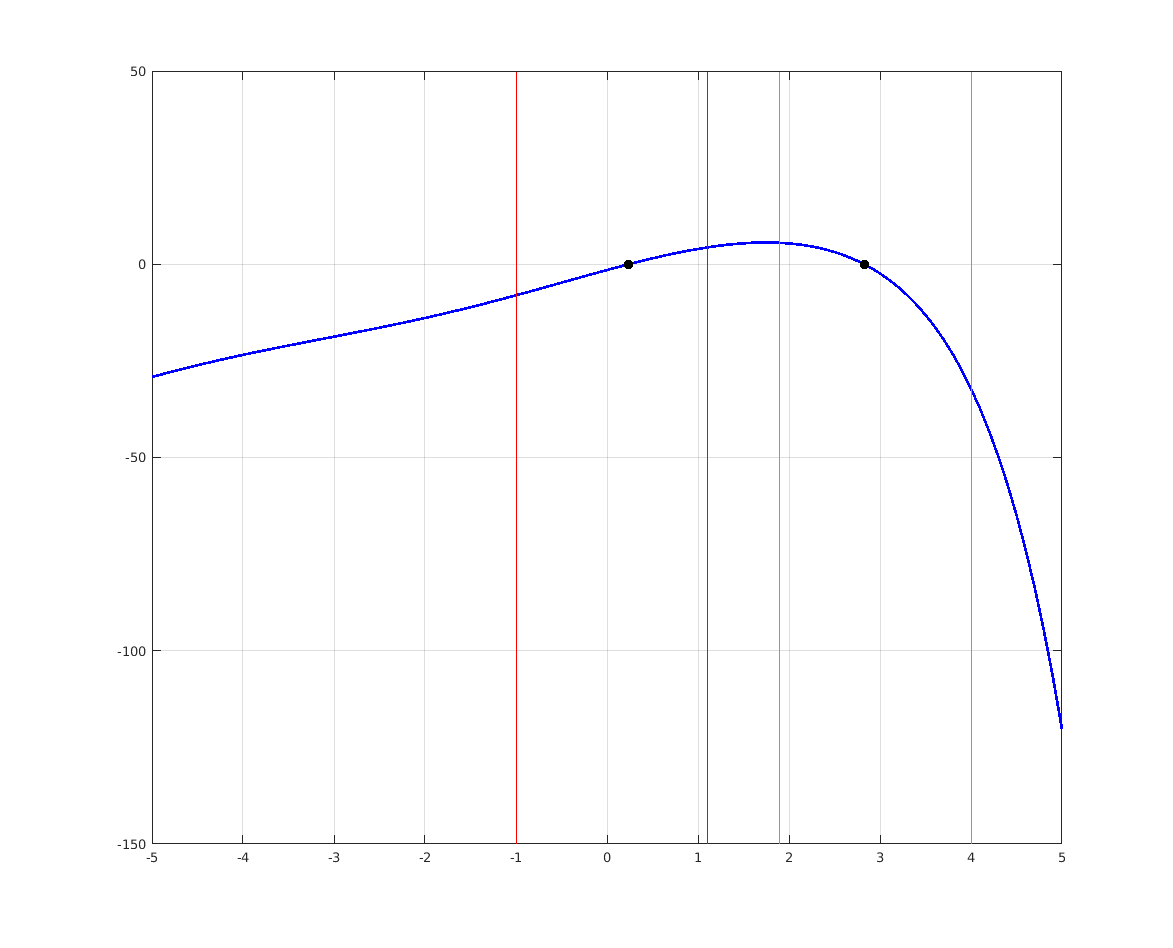
\includegraphics[width=\textwidth]{1}
\end{figure}


\subsection{Skrypt generujący rozwiązanie zadania w programie Matlab}
\begin{lstlisting}
%Realizacja zadania 1
clear; 
%Generowanie wykresu funkcji aby sprawdzic poprwanosc otrzymanych rozwiazan 
x  = -5: .1 : 5;
plot(x, fun(x), 'b','LineWidth', 2)
grid on
axis([-5 5 -150 150])

n=100; 
x1 = -1; 
x2 = 0; 

%wyznaczanie przedzialow izolacji na podstawie wkryptu MNUM
for k=1:2
    for j=1:n
        if fun(x1)*fun(x2)<0
            a = x1;
            b = x2;
            fprintf('Wyniki dla %d miejsca zerowego w przedziale [%d,%d]\n',k,a,b);
            bisection('fun',a,b,100);
            secant('fun',a,b,100);
            newton('fun',a,100);
            x1 = 3; 
            x2 = 4; 
            break;
        elseif abs(fun(x1))<abs(fun(x2))
            x1 = x1+1.1*(x1-x2);
        else
            x2 = x2+1.1*(x2-x1);
        end
        if(x1>5)&&(x2<(-5))
            break; %wyjscie z petli po przekroczeniu przedzialu
        end
    end
end
\end{lstlisting}
\vspace{1cm}


\subsection{Wyniki}

\begin{table}[H]
\centering
\label{my-label}
\begin{tabular}{llll}
\hline
\multicolumn{4}{c}{\textbf{Metoda siecznych pierwsze miejsce zerowe}} \\ \hline
\multicolumn{1}{|l|}{\textbf{iteracja}} & \multicolumn{1}{l|}{\textbf{przedział}} & \multicolumn{1}{l|}{\textbf{wynik}} & \multicolumn{1}{l|}{\textbf{wartość funkcji}} \\ \hline
\multicolumn{1}{|l|}{1} & \multicolumn{1}{l|}{{[}1.1000000000;0.3637775411{]}} & \multicolumn{1}{l|}{0.3637775410734196} & \multicolumn{1}{l|}{7.362e-01} \\ \hline
\multicolumn{1}{|l|}{2} & \multicolumn{1}{l|}{{[}0.3637775411;0.2120880091{]}} & \multicolumn{1}{l|}{0.2120880090516735} & \multicolumn{1}{l|}{1.517e-01} \\ \hline
\multicolumn{1}{|l|}{3} & \multicolumn{1}{l|}{{[}0.2120880091;0.2402303125{]}} & \multicolumn{1}{l|}{0.2402303124756739} & \multicolumn{1}{l|}{-2.814e-02} \\ \hline
\multicolumn{1}{|l|}{4} & \multicolumn{1}{l|}{{[}0.2402303125;0.2397497010{]}} & \multicolumn{1}{l|}{0.2397497010094280} & \multicolumn{1}{l|}{4.806e-04} \\ \hline
\multicolumn{1}{|l|}{5} & \multicolumn{1}{l|}{{[}0.2397497010;0.2397479765{]}} & \multicolumn{1}{l|}{0.2397479764875909} & \multicolumn{1}{l|}{1.725e-06} \\ \hline
\multicolumn{1}{|l|}{6} & \multicolumn{1}{l|}{{[}0.2397479765;0.2397479766{]}} & \multicolumn{1}{l|}{0.2397479765971351} & \multicolumn{1}{l|}{-1.095e-10} \\ \hline
\multicolumn{1}{|l|}{7} & \multicolumn{1}{l|}{{[}0.2397479766;0.2397479766{]}} & \multicolumn{1}{l|}{0.2397479765971350} & \multicolumn{1}{l|}{3.647e-17} \\ \hline
\multicolumn{1}{|l|}{8} & \multicolumn{1}{l|}{{[}0.2397479766;0.2397479766{]}} & \multicolumn{1}{l|}{0.2397479765971350} & \multicolumn{1}{l|}{0.000e+00} \\ \hline
\end{tabular}
\end{table}

\begin{table}[H]
\centering
\label{my-label}
\begin{tabular}{llll}
\hline
\multicolumn{4}{c}{\textbf{Metoda siecznych drugie miejsce zerowe}} \\ \hline
\multicolumn{1}{|l|}{\textbf{iteracja}} & \multicolumn{1}{l|}{\textbf{przedział}} & \multicolumn{1}{l|}{\textbf{wynik}} & \multicolumn{1}{l|}{\textbf{wartość funkcji}} \\ \hline
\multicolumn{1}{|l|}{1} & \multicolumn{1}{l|}{{[}4.0000000000;2.2085621561{]}} & \multicolumn{1}{l|}{2.2085621561012472} & \multicolumn{1}{l|}{1.791e+00} \\ \hline
\multicolumn{1}{|l|}{2} & \multicolumn{1}{l|}{{[}2.2085621561;2.4401148217{]}} & \multicolumn{1}{l|}{2.4401148217298374} & \multicolumn{1}{l|}{-2.316e-01} \\ \hline
\multicolumn{1}{|l|}{3} & \multicolumn{1}{l|}{{[}2.4401148217;3.1268105849{]}} & \multicolumn{1}{l|}{3.1268105848860621} & \multicolumn{1}{l|}{-6.867e-01} \\ \hline
\multicolumn{1}{|l|}{4} & \multicolumn{1}{l|}{{[}3.1268105849;2.7431506522{]}} & \multicolumn{1}{l|}{2.7431506521755535} & \multicolumn{1}{l|}{3.837e-01} \\ \hline
\multicolumn{1}{|l|}{5} & \multicolumn{1}{l|}{{[}2.7431506522;2.8107252731{]}} & \multicolumn{1}{l|}{2.8107252730503189} & \multicolumn{1}{l|}{-6.757e-02} \\ \hline
\multicolumn{1}{|l|}{6} & \multicolumn{1}{l|}{{[}2.8107252731;2.8280523947{]}} & \multicolumn{1}{l|}{2.8280523946681111} & \multicolumn{1}{l|}{-1.733e-02} \\ \hline
\multicolumn{1}{|l|}{7} & \multicolumn{1}{l|}{{[}2.8280523947;2.8270291416{]}} & \multicolumn{1}{l|}{2.8270291416146467} & \multicolumn{1}{l|}{1.023e-03} \\ \hline
\multicolumn{1}{|l|}{8} & \multicolumn{1}{l|}{{[}2.8270291416;2.8270409015{]}} & \multicolumn{1}{l|}{2.8270409014519227} & \multicolumn{1}{l|}{-1.176e-05} \\ \hline
\multicolumn{1}{|l|}{9} & \multicolumn{1}{l|}{{[}2.8270409015;2.8270409099{]}} & \multicolumn{1}{l|}{2.8270409098837272} & \multicolumn{1}{l|}{-8.432e-09} \\ \hline
\multicolumn{1}{|l|}{10} & \multicolumn{1}{l|}{{[}2.8270409099;2.8270409099{]}} & \multicolumn{1}{l|}{2.8270409098836571} & \multicolumn{1}{l|}{7.003e-14} \\ \hline
\multicolumn{1}{|l|}{11} & \multicolumn{1}{l|}{{[}2.8270409099;2.8270409099{]}} & \multicolumn{1}{l|}{2.8270409098836571} & \multicolumn{1}{l|}{-0.000e+00} \\ \hline
\end{tabular}
\end{table}

\begin{table}[H]
\centering
\label{my-label}
\begin{tabular}{llll}
\hline
\multicolumn{4}{c}{\textbf{Metoda Newtona pierwsze miejsce zerowe}} \\ \hline
\multicolumn{1}{|l|}{\textbf{iteracja}} & \multicolumn{1}{l|}{\textbf{przedział}} & \multicolumn{1}{l|}{\textbf{wynik}} & \multicolumn{1}{l|}{\textbf{wartość funkcji}} \\ \hline
\multicolumn{1}{|l|}{1} & \multicolumn{1}{l|}{-1.2594323665} & \multicolumn{1}{l|}{0.2594323664525493} & \multicolumn{1}{l|}{-8.046e+00} \\ \hline
\multicolumn{1}{|l|}{2} & \multicolumn{1}{l|}{0.0197367824} & \multicolumn{1}{l|}{0.2396955840431176} & \multicolumn{1}{l|}{1.195e-01} \\ \hline
\multicolumn{1}{|l|}{3} & \multicolumn{1}{l|}{-0.0000523922} & \multicolumn{1}{l|}{0.2397479762357552} & \multicolumn{1}{l|}{-3.190e-04} \\ \hline
\multicolumn{1}{|l|}{4} & \multicolumn{1}{l|}{-0.0000000004} & \multicolumn{1}{l|}{0.2397479765971350} & \multicolumn{1}{l|}{-2.200e-09} \\ \hline
\multicolumn{1}{|l|}{5} & \multicolumn{1}{l|}{0.0000000000} & \multicolumn{1}{l|}{0.2397479765971350} & \multicolumn{1}{l|}{0.000e+00} \\ \hline
\end{tabular}
\end{table}

\begin{table}[H]
\centering
\label{my-label}
\begin{tabular}{llll}
\hline
\multicolumn{4}{c}{\textbf{Metoda Newtona drugie miejsce zerowe}} \\ \hline
\multicolumn{1}{|l|}{\textbf{iteracja}} & \multicolumn{1}{l|}{\textbf{przedział}} & \multicolumn{1}{l|}{\textbf{wynik}} & \multicolumn{1}{l|}{\textbf{wartość funkcji}} \\ \hline
\multicolumn{1}{|l|}{1} & \multicolumn{1}{l|}{-4.8651088967} & \multicolumn{1}{l|}{6.7651088967106006} & \multicolumn{1}{l|}{5.539e+00} \\ \hline
\multicolumn{1}{|l|}{2} & \multicolumn{1}{l|}{0.9610395411} & \multicolumn{1}{l|}{5.8040693556058418} & \multicolumn{1}{l|}{-8.263e+02} \\ \hline
\multicolumn{1}{|l|}{3} & \multicolumn{1}{l|}{0.9185069972} & \multicolumn{1}{l|}{4.8855623584001924} & \multicolumn{1}{l|}{-2.980e+02} \\ \hline
\multicolumn{1}{|l|}{4} & \multicolumn{1}{l|}{0.8319658399} & \multicolumn{1}{l|}{4.0535965184699823} & \multicolumn{1}{l|}{-1.049e+02} \\ \hline
\multicolumn{1}{|l|}{5} & \multicolumn{1}{l|}{0.6650562218} & \multicolumn{1}{l|}{3.3885402966240363} & \multicolumn{1}{l|}{-3.489e+01} \\ \hline
\multicolumn{1}{|l|}{6} & \multicolumn{1}{l|}{0.4056676310} & \multicolumn{1}{l|}{2.9828726656584705} & \multicolumn{1}{l|}{-1.013e+01} \\ \hline
\multicolumn{1}{|l|}{7} & \multicolumn{1}{l|}{0.1405409130} & \multicolumn{1}{l|}{2.8423317526851513} & \multicolumn{1}{l|}{-2.126e+00} \\ \hline
\multicolumn{1}{|l|}{8} & \multicolumn{1}{l|}{0.0151272015} & \multicolumn{1}{l|}{2.8272045512095620} & \multicolumn{1}{l|}{-1.890e-01} \\ \hline
\multicolumn{1}{|l|}{9} & \multicolumn{1}{l|}{0.0001636224} & \multicolumn{1}{l|}{2.8270409288572882} & \multicolumn{1}{l|}{-2.001e-03} \\ \hline
\multicolumn{1}{|l|}{10} & \multicolumn{1}{l|}{0.0000000190} & \multicolumn{1}{l|}{2.8270409098836575} & \multicolumn{1}{l|}{-2.320e-07} \\ \hline
\multicolumn{1}{|l|}{11} & \multicolumn{1}{l|}{0.0000000000} & \multicolumn{1}{l|}{2.8270409098836571} & \multicolumn{1}{l|}{-3.553e-15} \\ \hline
\multicolumn{1}{|l|}{12} & \multicolumn{1}{l|}{-0.0000000000} & \multicolumn{1}{l|}{2.8270409098836571} & \multicolumn{1}{l|}{0.000e+00} \\ \hline
\end{tabular}
\end{table}

\begin{table}[H]
\centering
\label{my-label}
\begin{tabular}{llll}
\hline
\multicolumn{4}{c}{\textbf{Metoda bisekcji pierwsze miejsce zerowe}} \\ \hline
\multicolumn{1}{|l|}{\textbf{iteracja}} & \multicolumn{1}{l|}{\textbf{przedział}} & \multicolumn{1}{l|}{\textbf{wynik}} & \multicolumn{1}{l|}{\textbf{wartość funkcji}} \\ \hline
\multicolumn{1}{|l|}{1} & \multicolumn{1}{l|}{{[}-1.0000000000;1.1000000000{]}} & \multicolumn{1}{l|}{0.0500000000000000} & \multicolumn{1}{l|}{-1.181e+00} \\ \hline
\multicolumn{1}{|l|}{2} & \multicolumn{1}{l|}{{[}0.0500000000;1.1000000000{]}} & \multicolumn{1}{l|}{0.5750000000000001} & \multicolumn{1}{l|}{1.934e+00} \\ \hline
\multicolumn{1}{|l|}{3} & \multicolumn{1}{l|}{{[}0.0500000000;0.5750000000{]}} & \multicolumn{1}{l|}{0.3125000000000001} & \multicolumn{1}{l|}{4.386e-01} \\ \hline
\multicolumn{1}{|l|}{4} & \multicolumn{1}{l|}{{[}0.0500000000;0.3125000000{]}} & \multicolumn{1}{l|}{0.1812500000000000} & \multicolumn{1}{l|}{-3.589e-01} \\ \hline
\multicolumn{1}{|l|}{5} & \multicolumn{1}{l|}{{[}0.1812500000;0.3125000000{]}} & \multicolumn{1}{l|}{0.2468750000000001} & \multicolumn{1}{l|}{4.336e-02} \\ \hline
\multicolumn{1}{|l|}{6} & \multicolumn{1}{l|}{{[}0.1812500000;0.2468750000{]}} & \multicolumn{1}{l|}{0.2140625000000000} & \multicolumn{1}{l|}{-1.569e-01} \\ \hline
\multicolumn{1}{|l|}{7} & \multicolumn{1}{l|}{{[}0.2140625000;0.2468750000{]}} & \multicolumn{1}{l|}{0.2304687500000001} & \multicolumn{1}{l|}{-5.657e-02} \\ \hline
\multicolumn{1}{|l|}{8} & \multicolumn{1}{l|}{{[}0.2304687500;0.2468750000{]}} & \multicolumn{1}{l|}{0.2386718750000001} & \multicolumn{1}{l|}{-6.553e-03} \\ \hline
\multicolumn{1}{|l|}{9} & \multicolumn{1}{l|}{{[}0.2386718750;0.2468750000{]}} & \multicolumn{1}{l|}{0.2427734375000001} & \multicolumn{1}{l|}{1.841e-02} \\ \hline
\multicolumn{1}{|l|}{10} & \multicolumn{1}{l|}{{[}0.2386718750;0.2427734375{]}} & \multicolumn{1}{l|}{0.2407226562500001} & \multicolumn{1}{l|}{5.934e-03} \\ \hline
\multicolumn{1}{|l|}{11} & \multicolumn{1}{l|}{{[}0.2386718750;0.2407226563{]}} & \multicolumn{1}{l|}{0.2396972656250000} & \multicolumn{1}{l|}{-3.088e-04} \\ \hline
\multicolumn{1}{|l|}{12} & \multicolumn{1}{l|}{{[}0.2396972656;0.2407226563{]}} & \multicolumn{1}{l|}{0.2402099609375000} & \multicolumn{1}{l|}{2.813e-03} \\ \hline
\multicolumn{1}{|l|}{13} & \multicolumn{1}{l|}{{[}0.2396972656;0.2402099609{]}} & \multicolumn{1}{l|}{0.2399536132812500} & \multicolumn{1}{l|}{1.252e-03} \\ \hline
\multicolumn{1}{|l|}{14} & \multicolumn{1}{l|}{{[}0.2396972656;0.2399536133{]}} & \multicolumn{1}{l|}{0.2398254394531250} & \multicolumn{1}{l|}{4.717e-04} \\ \hline
\multicolumn{1}{|l|}{15} & \multicolumn{1}{l|}{{[}0.2396972656;0.2398254395{]}} & \multicolumn{1}{l|}{0.2397613525390626} & \multicolumn{1}{l|}{8.145e-05} \\ \hline
\multicolumn{1}{|l|}{16} & \multicolumn{1}{l|}{{[}0.2396972656;0.2397613525{]}} & \multicolumn{1}{l|}{0.2397293090820313} & \multicolumn{1}{l|}{-1.137e-04} \\ \hline
\multicolumn{1}{|l|}{17} & \multicolumn{1}{l|}{{[}0.2397293091;0.2397613525{]}} & \multicolumn{1}{l|}{0.2397453308105469} & \multicolumn{1}{l|}{-1.611e-05} \\ \hline
\multicolumn{1}{|l|}{18} & \multicolumn{1}{l|}{{[}0.2397453308;0.2397613525{]}} & \multicolumn{1}{l|}{0.2397533416748047} & \multicolumn{1}{l|}{3.267e-05} \\ \hline
\multicolumn{1}{|l|}{19} & \multicolumn{1}{l|}{{[}0.2397453308;0.2397533417{]}} & \multicolumn{1}{l|}{0.2397493362426759} & \multicolumn{1}{l|}{8.279e-06} \\ \hline
\multicolumn{1}{|l|}{20} & \multicolumn{1}{l|}{{[}0.2397453308;0.2397493362{]}} & \multicolumn{1}{l|}{0.2397473335266114} & \multicolumn{1}{l|}{-3.916e-06} \\ \hline
\multicolumn{1}{|l|}{21} & \multicolumn{1}{l|}{{[}0.2397473335;0.2397493362{]}} & \multicolumn{1}{l|}{0.2397483348846436} & \multicolumn{1}{l|}{2.182e-06} \\ \hline
\multicolumn{1}{|l|}{22} & \multicolumn{1}{l|}{{[}0.2397473335;0.2397483349{]}} & \multicolumn{1}{l|}{0.2397478342056275} & \multicolumn{1}{l|}{-8.670e-07} \\ \hline
\multicolumn{1}{|l|}{23} & \multicolumn{1}{l|}{{[}0.2397478342;0.2397483349{]}} & \multicolumn{1}{l|}{0.2397480845451356} & \multicolumn{1}{l|}{6.573e-07} \\ \hline
\multicolumn{1}{|l|}{24} & \multicolumn{1}{l|}{{[}0.2397478342;0.2397480845{]}} & \multicolumn{1}{l|}{0.2397479593753815} & \multicolumn{1}{l|}{-1.049e-07} \\ \hline
\multicolumn{1}{|l|}{25} & \multicolumn{1}{l|}{{[}0.2397479594;0.2397480845{]}} & \multicolumn{1}{l|}{0.2397480219602586} & \multicolumn{1}{l|}{2.762e-07} \\ \hline
\multicolumn{1}{|l|}{26} & \multicolumn{1}{l|}{{[}0.2397479594;0.2397480220{]}} & \multicolumn{1}{l|}{0.2397479906678200} & \multicolumn{1}{l|}{8.568e-08} \\ \hline
\multicolumn{1}{|l|}{27} & \multicolumn{1}{l|}{{[}0.2397479594;0.2397479907{]}} & \multicolumn{1}{l|}{0.2397479750216008} & \multicolumn{1}{l|}{-9.593e-09} \\ \hline
\multicolumn{1}{|l|}{28} & \multicolumn{1}{l|}{{[}0.2397479750;0.2397479907{]}} & \multicolumn{1}{l|}{0.2397479828447104} & \multicolumn{1}{l|}{3.804e-08} \\ \hline
\multicolumn{1}{|l|}{29} & \multicolumn{1}{l|}{{[}0.2397479750;0.2397479828{]}} & \multicolumn{1}{l|}{0.2397479789331556} & \multicolumn{1}{l|}{1.422e-08} \\ \hline
\multicolumn{1}{|l|}{30} & \multicolumn{1}{l|}{{[}0.2397479750;0.2397479789{]}} & \multicolumn{1}{l|}{0.2397479769773782} & \multicolumn{1}{l|}{2.315e-09} \\ \hline
\multicolumn{1}{|l|}{31} & \multicolumn{1}{l|}{{[}0.2397479750;0.2397479770{]}} & \multicolumn{1}{l|}{0.2397479759994895} & \multicolumn{1}{l|}{-3.639e-09} \\ \hline
\multicolumn{1}{|l|}{32} & \multicolumn{1}{l|}{{[}0.2397479760;0.2397479770{]}} & \multicolumn{1}{l|}{0.2397479764884338} & \multicolumn{1}{l|}{-6.619e-10} \\ \hline
\multicolumn{1}{|l|}{33} & \multicolumn{1}{l|}{{[}0.2397479765;0.2397479770{]}} & \multicolumn{1}{l|}{0.2397479767329060} & \multicolumn{1}{l|}{8.267e-10} \\ \hline
\multicolumn{1}{|l|}{34} & \multicolumn{1}{l|}{{[}0.2397479765;0.2397479767{]}} & \multicolumn{1}{l|}{0.2397479766106699} & \multicolumn{1}{l|}{8.241e-11} \\ \hline
\multicolumn{1}{|l|}{35} & \multicolumn{1}{l|}{{[}0.2397479765;0.2397479766{]}} & \multicolumn{1}{l|}{0.2397479765495519} & \multicolumn{1}{l|}{-2.897e-10} \\ \hline
\multicolumn{1}{|l|}{36} & \multicolumn{1}{l|}{{[}0.2397479765;0.2397479766{]}} & \multicolumn{1}{l|}{0.2397479765801109} & \multicolumn{1}{l|}{-1.037e-10} \\ \hline
\multicolumn{1}{|l|}{37} & \multicolumn{1}{l|}{{[}0.2397479766;0.2397479766{]}} & \multicolumn{1}{l|}{0.2397479765953904} & \multicolumn{1}{l|}{-1.062e-11} \\ \hline
\multicolumn{1}{|l|}{38} & \multicolumn{1}{l|}{{[}0.2397479766;0.2397479766{]}} & \multicolumn{1}{l|}{0.2397479766030302} & \multicolumn{1}{l|}{3.590e-11} \\ \hline
\multicolumn{1}{|l|}{39} & \multicolumn{1}{l|}{{[}0.2397479766;0.2397479766{]}} & \multicolumn{1}{l|}{0.2397479765992103} & \multicolumn{1}{l|}{1.264e-11} \\ \hline
\multicolumn{1}{|l|}{40} & \multicolumn{1}{l|}{{[}0.2397479766;0.2397479766{]}} & \multicolumn{1}{l|}{0.2397479765973003} & \multicolumn{1}{l|}{1.007e-12} \\ \hline
\multicolumn{1}{|l|}{41} & \multicolumn{1}{l|}{{[}0.2397479766;0.2397479766{]}} & \multicolumn{1}{l|}{0.2397479765963453} & \multicolumn{1}{l|}{-4.808e-12} \\ \hline
\multicolumn{1}{|l|}{42} & \multicolumn{1}{l|}{{[}0.2397479766;0.2397479766{]}} & \multicolumn{1}{l|}{0.2397479765968228} & \multicolumn{1}{l|}{-1.901e-12} \\ \hline
\multicolumn{1}{|l|}{43} & \multicolumn{1}{l|}{{[}0.2397479766;0.2397479766{]}} & \multicolumn{1}{l|}{0.2397479765970616} & \multicolumn{1}{l|}{-4.472e-13} \\ \hline
\multicolumn{1}{|l|}{44} & \multicolumn{1}{l|}{{[}0.2397479766;0.2397479766{]}} & \multicolumn{1}{l|}{0.2397479765971809} & \multicolumn{1}{l|}{2.796e-13} \\ \hline
\multicolumn{1}{|l|}{45} & \multicolumn{1}{l|}{{[}0.2397479766;0.2397479766{]}} & \multicolumn{1}{l|}{0.2397479765971213} & \multicolumn{1}{l|}{-8.371e-14} \\ \hline
\multicolumn{1}{|l|}{46} & \multicolumn{1}{l|}{{[}0.2397479766;0.2397479766{]}} & \multicolumn{1}{l|}{0.2397479765971511} & \multicolumn{1}{l|}{9.814e-14} \\ \hline
\multicolumn{1}{|l|}{47} & \multicolumn{1}{l|}{{[}0.2397479766;0.2397479766{]}} & \multicolumn{1}{l|}{0.2397479765971362} & \multicolumn{1}{l|}{7.105e-15} \\ \hline
\multicolumn{1}{|l|}{48} & \multicolumn{1}{l|}{{[}0.2397479766;0.2397479766{]}} & \multicolumn{1}{l|}{0.2397479765971287} & \multicolumn{1}{l|}{-3.830e-14} \\ \hline
\multicolumn{1}{|l|}{49} & \multicolumn{1}{l|}{{[}0.2397479766;0.2397479766{]}} & \multicolumn{1}{l|}{0.2397479765971325} & \multicolumn{1}{l|}{-1.521e-14} \\ \hline
\multicolumn{1}{|l|}{50} & \multicolumn{1}{l|}{{[}0.2397479766;0.2397479766{]}} & \multicolumn{1}{l|}{0.2397479765971343} & \multicolumn{1}{l|}{-3.997e-15} \\ \hline
\multicolumn{1}{|l|}{51} & \multicolumn{1}{l|}{{[}0.2397479766;0.2397479766{]}} & \multicolumn{1}{l|}{0.2397479765971353} & \multicolumn{1}{l|}{1.443e-15} \\ \hline
\multicolumn{1}{|l|}{52} & \multicolumn{1}{l|}{{[}0.2397479766;0.2397479766{]}} & \multicolumn{1}{l|}{0.2397479765971348} & \multicolumn{1}{l|}{-1.332e-15} \\ \hline
\multicolumn{1}{|l|}{53} & \multicolumn{1}{l|}{{[}0.2397479766;0.2397479766{]}} & \multicolumn{1}{l|}{0.2397479765971350} & \multicolumn{1}{l|}{0.000e+00} \\ \hline
\end{tabular}
\end{table}

\begin{table}[H]
\centering
\label{my-label}
\begin{tabular}{llll}
\hline
\multicolumn{4}{c}{\textbf{Metoda bisekcji drugie miejsce zerowe}} \\ \hline
\multicolumn{1}{|l|}{\textbf{iteracja}} & \multicolumn{1}{l|}{\textbf{przedział}} & \multicolumn{1}{l|}{\textbf{wynik}} & \multicolumn{1}{l|}{\textbf{wartość funkcji}} \\ \hline
\multicolumn{1}{|l|}{1} & \multicolumn{1}{l|}{{[}1.9000000000;4.0000000000{]}} & \multicolumn{1}{l|}{2.9500000000000002} & \multicolumn{1}{l|}{-1.639e+00} \\ \hline
\multicolumn{1}{|l|}{2} & \multicolumn{1}{l|}{{[}1.9000000000;2.9500000000{]}} & \multicolumn{1}{l|}{2.4249999999999998} & \multicolumn{1}{l|}{3.667e+00} \\ \hline
\multicolumn{1}{|l|}{3} & \multicolumn{1}{l|}{{[}2.4250000000;2.9500000000{]}} & \multicolumn{1}{l|}{2.6875000000000000} & \multicolumn{1}{l|}{1.544e+00} \\ \hline
\multicolumn{1}{|l|}{4} & \multicolumn{1}{l|}{{[}2.6875000000;2.9500000000{]}} & \multicolumn{1}{l|}{2.8187500000000001} & \multicolumn{1}{l|}{1.008e-01} \\ \hline
\multicolumn{1}{|l|}{5} & \multicolumn{1}{l|}{{[}2.8187500000;2.9500000000{]}} & \multicolumn{1}{l|}{2.8843750000000004} & \multicolumn{1}{l|}{-7.300e-01} \\ \hline
\multicolumn{1}{|l|}{6} & \multicolumn{1}{l|}{{[}2.8187500000;2.8843750000{]}} & \multicolumn{1}{l|}{2.8515625000000000} & \multicolumn{1}{l|}{-3.051e-01} \\ \hline
\multicolumn{1}{|l|}{7} & \multicolumn{1}{l|}{{[}2.8187500000;2.8515625000{]}} & \multicolumn{1}{l|}{2.8351562499999998} & \multicolumn{1}{l|}{-9.980e-02} \\ \hline
\multicolumn{1}{|l|}{8} & \multicolumn{1}{l|}{{[}2.8187500000;2.8351562500{]}} & \multicolumn{1}{l|}{2.8269531250000002} & \multicolumn{1}{l|}{1.073e-03} \\ \hline
\multicolumn{1}{|l|}{9} & \multicolumn{1}{l|}{{[}2.8269531250;2.8351562500{]}} & \multicolumn{1}{l|}{2.8310546875000000} & \multicolumn{1}{l|}{-4.922e-02} \\ \hline
\multicolumn{1}{|l|}{10} & \multicolumn{1}{l|}{{[}2.8269531250;2.8310546875{]}} & \multicolumn{1}{l|}{2.8290039062500001} & \multicolumn{1}{l|}{-2.403e-02} \\ \hline
\multicolumn{1}{|l|}{11} & \multicolumn{1}{l|}{{[}2.8269531250;2.8290039063{]}} & \multicolumn{1}{l|}{2.8279785156250004} & \multicolumn{1}{l|}{-1.147e-02} \\ \hline
\multicolumn{1}{|l|}{12} & \multicolumn{1}{l|}{{[}2.8269531250;2.8279785156{]}} & \multicolumn{1}{l|}{2.8274658203125003} & \multicolumn{1}{l|}{-5.197e-03} \\ \hline
\multicolumn{1}{|l|}{13} & \multicolumn{1}{l|}{{[}2.8269531250;2.8274658203{]}} & \multicolumn{1}{l|}{2.8272094726562500} & \multicolumn{1}{l|}{-2.061e-03} \\ \hline
\multicolumn{1}{|l|}{14} & \multicolumn{1}{l|}{{[}2.8269531250;2.8272094727{]}} & \multicolumn{1}{l|}{2.8270812988281251} & \multicolumn{1}{l|}{-4.938e-04} \\ \hline
\multicolumn{1}{|l|}{15} & \multicolumn{1}{l|}{{[}2.8269531250;2.8270812988{]}} & \multicolumn{1}{l|}{2.8270172119140629} & \multicolumn{1}{l|}{2.897e-04} \\ \hline
\multicolumn{1}{|l|}{16} & \multicolumn{1}{l|}{{[}2.8270172119;2.8270812988{]}} & \multicolumn{1}{l|}{2.8270492553710938} & \multicolumn{1}{l|}{-1.020e-04} \\ \hline
\multicolumn{1}{|l|}{17} & \multicolumn{1}{l|}{{[}2.8270172119;2.8270492554{]}} & \multicolumn{1}{l|}{2.8270332336425783} & \multicolumn{1}{l|}{9.385e-05} \\ \hline
\multicolumn{1}{|l|}{18} & \multicolumn{1}{l|}{{[}2.8270332336;2.8270492554{]}} & \multicolumn{1}{l|}{2.8270412445068360} & \multicolumn{1}{l|}{-4.091e-06} \\ \hline
\multicolumn{1}{|l|}{19} & \multicolumn{1}{l|}{{[}2.8270332336;2.8270412445{]}} & \multicolumn{1}{l|}{2.8270372390747074} & \multicolumn{1}{l|}{4.488e-05} \\ \hline
\multicolumn{1}{|l|}{20} & \multicolumn{1}{l|}{{[}2.8270372391;2.8270412445{]}} & \multicolumn{1}{l|}{2.8270392417907715} & \multicolumn{1}{l|}{2.040e-05} \\ \hline
\multicolumn{1}{|l|}{21} & \multicolumn{1}{l|}{{[}2.8270392418;2.8270412445{]}} & \multicolumn{1}{l|}{2.8270402431488035} & \multicolumn{1}{l|}{8.152e-06} \\ \hline
\multicolumn{1}{|l|}{22} & \multicolumn{1}{l|}{{[}2.8270402431;2.8270412445{]}} & \multicolumn{1}{l|}{2.8270407438278200} & \multicolumn{1}{l|}{2.030e-06} \\ \hline
\multicolumn{1}{|l|}{23} & \multicolumn{1}{l|}{{[}2.8270407438;2.8270412445{]}} & \multicolumn{1}{l|}{2.8270409941673282} & \multicolumn{1}{l|}{-1.031e-06} \\ \hline
\multicolumn{1}{|l|}{24} & \multicolumn{1}{l|}{{[}2.8270407438;2.8270409942{]}} & \multicolumn{1}{l|}{2.8270408689975741} & \multicolumn{1}{l|}{4.999e-07} \\ \hline
\multicolumn{1}{|l|}{25} & \multicolumn{1}{l|}{{[}2.8270408690;2.8270409942{]}} & \multicolumn{1}{l|}{2.8270409315824514} & \multicolumn{1}{l|}{-2.653e-07} \\ \hline
\multicolumn{1}{|l|}{26} & \multicolumn{1}{l|}{{[}2.8270408690;2.8270409316{]}} & \multicolumn{1}{l|}{2.8270409002900125} & \multicolumn{1}{l|}{1.173e-07} \\ \hline
\multicolumn{1}{|l|}{27} & \multicolumn{1}{l|}{{[}2.8270409003;2.8270409316{]}} & \multicolumn{1}{l|}{2.8270409159362320} & \multicolumn{1}{l|}{-7.400e-08} \\ \hline
\multicolumn{1}{|l|}{28} & \multicolumn{1}{l|}{{[}2.8270409003;2.8270409159{]}} & \multicolumn{1}{l|}{2.8270409081131223} & \multicolumn{1}{l|}{2.165e-08} \\ \hline
\multicolumn{1}{|l|}{29} & \multicolumn{1}{l|}{{[}2.8270409081;2.8270409159{]}} & \multicolumn{1}{l|}{2.8270409120246773} & \multicolumn{1}{l|}{-2.618e-08} \\ \hline
\multicolumn{1}{|l|}{30} & \multicolumn{1}{l|}{{[}2.8270409081;2.8270409120{]}} & \multicolumn{1}{l|}{2.8270409100688996} & \multicolumn{1}{l|}{-2.265e-09} \\ \hline
\multicolumn{1}{|l|}{31} & \multicolumn{1}{l|}{{[}2.8270409081;2.8270409101{]}} & \multicolumn{1}{l|}{2.8270409090910107} & \multicolumn{1}{l|}{9.691e-09} \\ \hline
\multicolumn{1}{|l|}{32} & \multicolumn{1}{l|}{{[}2.8270409091;2.8270409101{]}} & \multicolumn{1}{l|}{2.8270409095799551} & \multicolumn{1}{l|}{3.713e-09} \\ \hline
\multicolumn{1}{|l|}{33} & \multicolumn{1}{l|}{{[}2.8270409096;2.8270409101{]}} & \multicolumn{1}{l|}{2.8270409098244276} & \multicolumn{1}{l|}{7.242e-10} \\ \hline
\multicolumn{1}{|l|}{34} & \multicolumn{1}{l|}{{[}2.8270409098;2.8270409101{]}} & \multicolumn{1}{l|}{2.8270409099466636} & \multicolumn{1}{l|}{-7.704e-10} \\ \hline
\multicolumn{1}{|l|}{35} & \multicolumn{1}{l|}{{[}2.8270409098;2.8270409099{]}} & \multicolumn{1}{l|}{2.8270409098855458} & \multicolumn{1}{l|}{-2.310e-11} \\ \hline
\multicolumn{1}{|l|}{36} & \multicolumn{1}{l|}{{[}2.8270409098;2.8270409099{]}} & \multicolumn{1}{l|}{2.8270409098549867} & \multicolumn{1}{l|}{3.505e-10} \\ \hline
\multicolumn{1}{|l|}{37} & \multicolumn{1}{l|}{{[}2.8270409099;2.8270409099{]}} & \multicolumn{1}{l|}{2.8270409098702665} & \multicolumn{1}{l|}{1.637e-10} \\ \hline
\multicolumn{1}{|l|}{38} & \multicolumn{1}{l|}{{[}2.8270409099;2.8270409099{]}} & \multicolumn{1}{l|}{2.8270409098779061} & \multicolumn{1}{l|}{7.032e-11} \\ \hline
\multicolumn{1}{|l|}{39} & \multicolumn{1}{l|}{{[}2.8270409099;2.8270409099{]}} & \multicolumn{1}{l|}{2.8270409098817257} & \multicolumn{1}{l|}{2.361e-11} \\ \hline
\multicolumn{1}{|l|}{40} & \multicolumn{1}{l|}{{[}2.8270409099;2.8270409099{]}} & \multicolumn{1}{l|}{2.8270409098836358} & \multicolumn{1}{l|}{2.629e-13} \\ \hline
\multicolumn{1}{|l|}{41} & \multicolumn{1}{l|}{{[}2.8270409099;2.8270409099{]}} & \multicolumn{1}{l|}{2.8270409098845910} & \multicolumn{1}{l|}{-1.142e-11} \\ \hline
\multicolumn{1}{|l|}{42} & \multicolumn{1}{l|}{{[}2.8270409099;2.8270409099{]}} & \multicolumn{1}{l|}{2.8270409098841132} & \multicolumn{1}{l|}{-5.578e-12} \\ \hline
\multicolumn{1}{|l|}{43} & \multicolumn{1}{l|}{{[}2.8270409099;2.8270409099{]}} & \multicolumn{1}{l|}{2.8270409098838742} & \multicolumn{1}{l|}{-2.650e-12} \\ \hline
\multicolumn{1}{|l|}{44} & \multicolumn{1}{l|}{{[}2.8270409099;2.8270409099{]}} & \multicolumn{1}{l|}{2.8270409098837552} & \multicolumn{1}{l|}{-1.201e-12} \\ \hline
\multicolumn{1}{|l|}{45} & \multicolumn{1}{l|}{{[}2.8270409099;2.8270409099{]}} & \multicolumn{1}{l|}{2.8270409098836957} & \multicolumn{1}{l|}{-4.725e-13} \\ \hline
\multicolumn{1}{|l|}{46} & \multicolumn{1}{l|}{{[}2.8270409099;2.8270409099{]}} & \multicolumn{1}{l|}{2.8270409098836655} & \multicolumn{1}{l|}{-1.030e-13} \\ \hline
\multicolumn{1}{|l|}{47} & \multicolumn{1}{l|}{{[}2.8270409099;2.8270409099{]}} & \multicolumn{1}{l|}{2.8270409098836504} & \multicolumn{1}{l|}{8.171e-14} \\ \hline
\multicolumn{1}{|l|}{48} & \multicolumn{1}{l|}{{[}2.8270409099;2.8270409099{]}} & \multicolumn{1}{l|}{2.8270409098836580} & \multicolumn{1}{l|}{-1.066e-14} \\ \hline
\multicolumn{1}{|l|}{49} & \multicolumn{1}{l|}{{[}2.8270409099;2.8270409099{]}} & \multicolumn{1}{l|}{2.8270409098836540} & \multicolumn{1}{l|}{3.908e-14} \\ \hline
\multicolumn{1}{|l|}{50} & \multicolumn{1}{l|}{{[}2.8270409099;2.8270409099{]}} & \multicolumn{1}{l|}{2.8270409098836558} & \multicolumn{1}{l|}{1.421e-14} \\ \hline
\multicolumn{1}{|l|}{51} & \multicolumn{1}{l|}{{[}2.8270409099;2.8270409099{]}} & \multicolumn{1}{l|}{2.8270409098836566} & \multicolumn{1}{l|}{3.553e-15} \\ \hline
\multicolumn{1}{|l|}{52} & \multicolumn{1}{l|}{{[}2.8270409099;2.8270409099{]}} & \multicolumn{1}{l|}{2.8270409098836575} & \multicolumn{1}{l|}{-3.553e-15} \\ \hline
\multicolumn{1}{|l|}{53} & \multicolumn{1}{l|}{{[}2.8270409099;2.8270409099{]}} & \multicolumn{1}{l|}{2.8270409098836571} & \multicolumn{1}{l|}{0.000e+00} \\ \hline
\end{tabular}
\end{table}






\subsection{Wnioski}
Analizując wykres funkcji danej w zadanu możemy wstępnie okreslić miejsca zerowe i zachowanie funkcji w ich otoczeniu. Rozpatrywana funkcja posiada dwa rodzaje miejsc zerowych które mają wpływ na szybkość ich wyznaczania, ponieważ w otoczeniu jednego z nich funkcja jest nachylona pod małym kątem do osi X natomiast w przypadku drugiego miejsca obserwujemy duży lokakny przyrost, więc wykres funkcji jest mniej odchylony od osi pionowej. Jak wynika z otrzymanych rezultatów metoda bisekcji w obu przypadkach potrzebowała stosunkowo dużej ilości iteracji aby osiągnać zadaną dokładność. Jej zaletami jest niewrażliwość na szczególne zachowania funkcji więc mimo słabej zbierzności nadaje się do wyznaczania miejsc zerowych funkcji których przebiegu nie znamy w celu zabezpieczenia przez niezbierznością. Metoda siecznych potrzebowała około 10 iteracji aby dojść do wyniku. W przypadku wyznaczania miejsca zerowego w otoczeniu którego mamy doczynienia z płaską funkcją, jak miało to miejsze w drugim miejscu zerowym, metoda okazuje się najlepsza spośród wszystkich zastosowanych. Jej wadą jest niezbieżność w przypadku gdy sieczna przetnie wykres funkcji w większej ilości miejsc niż 2. Dlatego najeży wybierać wąskie przedziały startowe co zostsało uczynine w rozwiązaniu. Ostatnią wypróbowaną metodą jest metoda Newtona (stycznych), która w przypadku dobrego uwarunkowania (wąski przedział, brak odcinków o pochodniej mniejszej niż zero w przedziale startowym) okazuje się być najszybsza (w zadaniu ok 3-4 iteracje). Wynika to z najwyższego współczynnika zbierzności. W przypadku wyznaczania drugiego miejsca zerowego metodą Newtona rozpatrywany przedział zawierał fragment funkcji z ujemną pochodną. Spowodowało to zwiększenie liczby iteracji dla metody Newtona co można uznać za przypadek kiedy funkcja zawiodła. 


\section{Zadanie 2}

\subsection{Polecenie}
Używając metody Mullera MM2, proszę znaleźć wszystkie pierwiastki rzeczywiste i zespolone wielomianu
\begin{center}
$f(x) = a_{4}x^4+a_{3}x^3+a_{2}x^2+a_{1}x+a_{0}$ 
$
\left[
\begin{array}{ccccc}
       a_{4} & a_{3} & a_{2} & a_{1} & a_{0}
\end{array}
\right]
=
\left[
\begin{array}{ccccc}
       1 & 2 & 4 & -1 & 8
\end{array}
\right]$
\end{center}



\subsection{Metoda Mullera MM2}
Metoda Mullera polega na przybliżeniu rozpatrywanej funkcji trójmianem kwadratowym w otoczeniu zera i na tej podstawie wyznaczenia miejsc zerowych rzeczywistych bądź zespolonych. Wyróżniamy dwa rodzaje metody Mullera. Pierwsza (MM1) polega na aproksymacji wielomianu na podstawie jego wartości w 3 różnych punktach, natomiast druga (MM2) wykorzystuje wartość funkcji, pierwszej oraz drugiej pochodniej w danym punkcie i na tej podstawie zostają wyznaczone współczynniki $a$, $b$ ,$c$ trójmianu kwadratowego. Służą do tego następujące zależności:
\begin{center}
$y(0) = c = f(x_{k}),$
$y'(0) = b = f'(x_{k}),$
$y''(0) = 2a = f''(x_{k})$
\end{center}
Mając wyznaczone współczynniki trójmianu kwadratowego możemy bezpośrednio przejść do wzorów na jego pierwiastki:
\begin{center}
$z_{1} = \frac{-2f(x_{k})}{f'(x_{k})+\sqrt{(f'(x_{k}))^2-2f(x_{k})f''(x_{k})}}$
\end{center}
\begin{center}
$z_{2} = \frac{-2f(x_{k})}{f'(x_{k})-\sqrt{(f'(x_{k}))^2-2f(x_{k})f''(x_{k})}}$
\end{center}
Przeprowadzając iteracyjne przybliżanie zera wybieramy pierwiastek o mniejszym module:
\begin{center}
$x_{k+1} = x_{k}+min(|z_{1}|,|z_{2}|)$
\end{center}
Metoda Mullera podobnie jak Newtona jest zbierzna jedynie lokalnie z rzędem zbierzności 1.84. Jest szybsza od metody siecznych i niewiele wolniejsza od metody Newtona. Znaczącą różnicą jest implementacja pozwalająca na wyznaczanie zespolonych zer funkcji. 


\subsection{Realizacja w programie Matlab}
\begin{lstlisting}
function [value] = df(x,n)
%DF funkcja zwracajaca wyanaczona alanlitycznie pochodna wielomianu
%danego w zadaniu. 
%x - argument
%n  - 0-wartosac funkcji,1-pierwsza pochodna,2-druga pochodna
% f(x) = x^4+3x^3-8x^2+4x+2
% f'(x) = 4x^3+9x^2-16x+4
% f''(x) = 12x^2+18x-16
    if n == 0
        value = x.^4+3*x.^3-8*x.^2+4*x+2; 
    elseif n == 1
        value = 4*x.^3+9*x.^2-16*x+4;
    elseif n == 2
        value = 12*x.^2+18*x-16;
    else
        value = 0; 
    end
end

function [z] = muller(x,n)
%Funkcja zwracajaca wektor pierwiastkow rzeczywistych wielomianu
%danego w zadaniu
%A - wektor wspolczynnikow wielomianu
%x - punkt startowy
%n - ilosc iteracji
    %z = (1:n); 
    for i = 1:n
        %obliczamy mianowniki punktow w celu ich porownania
        z1 = df(x,1)+sqrt(df(x,1)^2-2*df(x,0)*df(x,2));
        z2 = df(x,1)-sqrt(df(x,1)^2-2*df(x,0)*df(x,2)); 
    
        if abs(z1) > abs(z2)
            zmin = -2*df(x,0)/z1; 
        else 
            zmin = -2*df(x,0)/z2;
        end 
        x = x+zmin; 
    end
    z = x; 
end

\end{lstlisting}

\vspace{1cm}

\subsection{Wyniki działania programu}

\begin{figure}[H]
\caption{Wykres wielomianu z zadania 2}
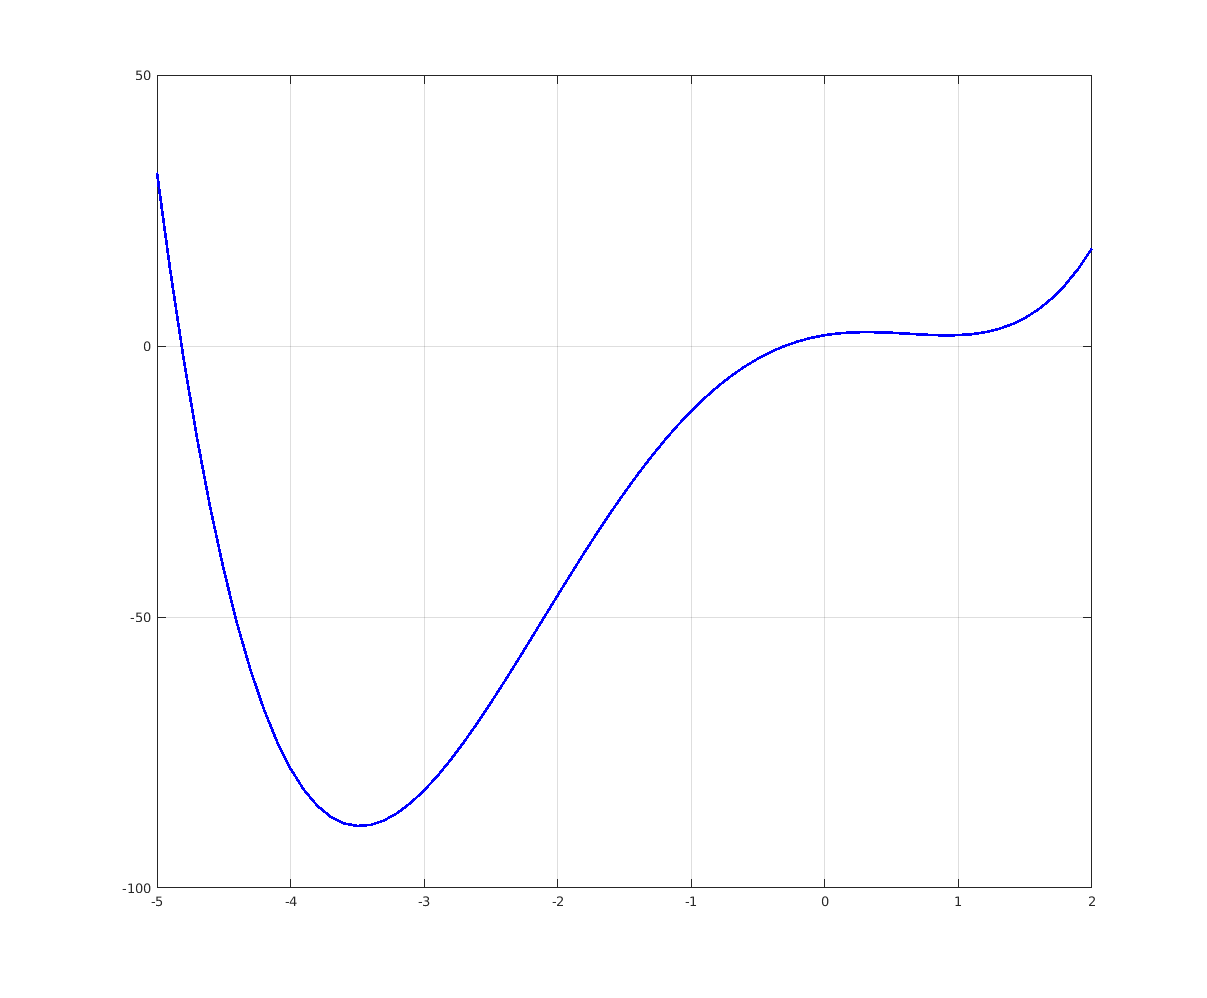
\includegraphics[width=\textwidth]{2}
\end{figure}

\begin{table}[H]
\centering
\label{my-label}
\begin{tabular}{|l|l|l|l|}
\hline
\multicolumn{4}{|c|}{\textbf{Miejsca zerowe wyznaczone alalitycznie}} \\ \hline
-4.8158 & -0.30075 & 1.05826 - 0.51087i & 1.05826 + 0.51087i \\ \hline
\multicolumn{4}{|c|}{\textbf{Miejsca zerowe wyznaczone metodą Mullera}} \\ \hline
-4.8158 & -0.3007 & 1.0583 - 0.5109i & 1.0583 + 0.5109i \\ \hline
\end{tabular}
\end{table}

\begin{table}[H]
\centering
\label{my-label}
\begin{tabular}{|l|l|l|l|}
\hline
\multicolumn{4}{|c|}{\textbf{Wyniki zadanie 2 cz. 1}} \\ \hline
\multicolumn{1}{|c|}{przedział startowy} & iteracja & wynik & przyrost \\ \hline
-5 & 1 & -4.815098 & 0.184902 \\ \hline
-5 & 2 & -4.815775 & -0.000677 \\ \hline
-5 & 3 & -4.815775 & 0.000000 \\ \hline
-5 & 4 & -4.815775 & 0.000000 \\ \hline
-5 & 5 & -4.815775 & -0.000000 \\ \hline
-5 & 6 & -4.815775 & 0.000000 \\ \hline
-4 & 1 & -4.872683 & -0.872683 \\ \hline
-4 & 2 & -4.815756 & 0.056927 \\ \hline
-4 & 3 & -4.815775 & -0.000019 \\ \hline
-4 & 4 & -4.815775 & 0.000000 \\ \hline
-4 & 5 & -4.815775 & 0.000000 \\ \hline
-4 & 6 & -4.815775 & -0.000000 \\ \hline
-3 & 1 & -1.478763 & 1.521237 \\ \hline
-3 & 2 & -0.472623 & 1.006140 \\ \hline
-3 & 3 & -0.300054 & 0.172569 \\ \hline
-3 & 4 & -0.300747 & -0.000693 \\ \hline
-3 & 5 & -0.300747 & 0.000000 \\ \hline
-3 & 6 & -0.300747 & -0.000000 \\ \hline
-2 & 1 & -0.774964 & 1.225036 \\ \hline
-2 & 2 & -0.296363 & 0.478601 \\ \hline
-2 & 3 & -0.300747 & -0.004383 \\ \hline
-2 & 4 & -0.300747 & 0.000000 \\ \hline
-2 & 5 & -0.300747 & -0.000000 \\ \hline
-2 & 6 & -0.300747 & -0.000000 \\ \hline
-1 & 1 & -0.311312 & 0.688688 \\ \hline
-1 & 2 & -0.300746 & 0.010565 \\ \hline
-1 & 3 & -0.300747 & -0.000000 \\ \hline
-1 & 4 & -0.300747 & -0.000000 \\ \hline
-1 & 5 & -0.300747 & -0.000000 \\ \hline
-1 & 6 & -0.300747 & -0.000000 \\ \hline
\end{tabular}
\end{table}

\begin{table}[H]
\centering
\label{my-label}
\begin{tabular}{|l|l|l|l|}
\hline
\multicolumn{4}{|c|}{\textbf{Wyniki zadanie 2 cz. 2}} \\ \hline
\multicolumn{1}{|c|}{przedział startowy} & iteracja & wynik & przyrost \\ \hline
0 & 1 & -0.309017 & -0.309017 \\ \hline
0 & 2 & -0.300747 & 0.008270 \\ \hline
0 & 3 & -0.300747 & -0.000000 \\ \hline
0 & 4 & -0.300747 & -0.000000 \\ \hline
0 & 5 & -0.300747 & -0.000000 \\ \hline
0 & 6 & -0.300747 & -0.000000 \\ \hline
1 & 1 & 0.928571 & -0.071429 \\ \hline
1 & 2 & 1.057209 & 0.128638 \\ \hline
1 & 3 & 1.058261 & 0.001052 \\ \hline
1 & 4 & 1.058261 & -0.000000 \\ \hline
1 & 5 & 1.058261 & -0.000000 \\ \hline
1 & 6 & 1.058261 & 0.000000 \\ \hline
2 & 1 & 1.411765 & -0.588235 \\ \hline
2 & 2 & 1.089902 & -0.321863 \\ \hline
2 & 3 & 1.058224 & -0.031678 \\ \hline
2 & 4 & 1.058261 & 0.000037 \\ \hline
2 & 5 & 1.058261 & 0.000000 \\ \hline
2 & 6 & 1.058261 & -0.000000 \\ \hline
3 & 1 & 2.006849 & -0.993151 \\ \hline
3 & 2 & 1.257315 & -0.749534 \\ \hline
3 & 3 & 1.044287 & -0.213028 \\ \hline
3 & 4 & 1.058128 & 0.013841 \\ \hline
3 & 5 & 1.058261 & 0.000133 \\ \hline
3 & 6 & 1.058261 & 0.000000 \\ \hline
4 & 1 & 2.629032 & -1.370968 \\ \hline
4 & 2 & 2.004778 & -0.624254 \\ \hline
4 & 3 & 1.414140 & -0.590638 \\ \hline
4 & 4 & 1.090117 & -0.324023 \\ \hline
4 & 5 & 1.058222 & -0.031896 \\ \hline
4 & 6 & 1.058261 & 0.000039 \\ \hline
\end{tabular}
\end{table}

\subsection{Wnioski}
Metoda Mullera dla wielomianu danego w zadaniu okazała się bardzo szybka, potrzebynch było jedynie kilka iteracji aby dojść do wyników zbliżonych do rozwiązania analitycznego. Komentarza wymaga realizacja zadania, ponieważ metoda została zastosowana kolejno do przedziałów o długości 1 rozpoczynając od pierwszego zawierającego zero funkcji (co zostało ustalone na podstawie obliczeń analitycznych). Dzięki aproksymacji kwadratowej metoda zawsze zbiegała do bliższego od wierzchołka paraboli zera, co uniwmożliwiło pominięcie rozwiązania podczas badania kolejnych przedziałów. Jeżeli chodzi o pierwiastki zespolone spełniają one warunek wzajemnego sprzężenia. Wszystkich rozwiązań wyszło tyle ile wynosi stopień wielomainu co równierz jest zgodne z teorią. 
	
\end{document}


